\documentclass[oneside, 11pt]{article}

\usepackage[T1]{fontenc}
\usepackage[utf8]{inputenc}
\usepackage[dutch]{babel}

\usepackage{fouriernc}
\usepackage[detect-all, load-configurations=binary,
            separate-uncertainty=true, per-mode=symbol,
            retain-explicit-plus, range-phrase={ tot }]{siunitx}

\usepackage{setspace}
\setstretch{1.2}

\setlength{\parskip}{\smallskipamount}
\setlength{\parindent}{0pt}

\usepackage{geometry}
\geometry{marginparwidth=0.5cm, verbose, a4paper, tmargin=3cm, bmargin=3cm, lmargin=2cm, rmargin=2cm}

\usepackage{float}

\usepackage[fleqn]{amsmath}
\numberwithin{equation}{section}
\numberwithin{figure}{section}

\usepackage{graphicx}
\graphicspath{{Figures/}}
\usepackage{subfig}

\usepackage{tikz}
\usetikzlibrary{plotmarks}

\usepackage{fancyhdr}
\pagestyle{fancy}
\fancyhf{}
\rhead{\thepage}
\renewcommand{\footrulewidth}{0pt}
\renewcommand{\headrulewidth}{0pt}

\usepackage{relsize}
\usepackage{xspace}
\usepackage{url}

\newcommand{\figref}[1]{Figuur~\ref{#1}}

\newcommand{\hisparc}{\textsmaller{HiSPARC}\xspace}
\newcommand{\kascade}{\textsmaller{KASCADE}\xspace}
\newcommand{\sapphire}{\textsmaller{SAPPHiRE}\xspace}
\newcommand{\jsparc}{\textsmaller{jSparc}\xspace}
\newcommand{\hdf}{\textsmaller{HDF5}\xspace}
\newcommand{\aires}{\textsmaller{AIRES}\xspace}
\newcommand{\csv}{\textsmaller{CSV}\xspace}
\newcommand{\python}{\textsmaller{PYTHON}\xspace}
\newcommand{\corsika}{\textsmaller{CORSIKA}\xspace}
\newcommand{\labview}{\textsmaller{LabVIEW}\xspace}
\newcommand{\daq}{\textsmaller{DAQ}\xspace}
\newcommand{\adc}{\textsmaller{ADC}\xspace}
\newcommand{\adcs}{\textsmaller{ADC}s\xspace}
\newcommand{\Adcs}{A\textsmaller{DC}s\xspace}
\newcommand{\hi}{\textsc{h i}\xspace}
\newcommand{\hii}{\textsc{h ii}\xspace}
\newcommand{\mip}{\textsmaller{MIP}\xspace}
\newcommand{\hisparcii}{\textsmaller{HiSPARC II}\xspace}
\newcommand{\hisparciii}{\textsmaller{HiSPARC III}\xspace}
\newcommand{\pmt}{\textsmaller{PMT}\xspace}
\newcommand{\pmts}{\textsmaller{PMT}s\xspace}

\DeclareSIUnit{\electronvolt}{\ensuremath{\mathrm{e\!\!\:V}}}

\DeclareSIUnit{\unitsigma}{\ensuremath{\sigma}}
\DeclareSIUnit{\mip}{\textsmaller{MIP}}
\DeclareSIUnit{\adc}{\textsmaller{ADC}}

\DeclareSIUnit{\gauss}{G}
\DeclareSIUnit{\parsec}{pc}
\DeclareSIUnit{\year}{yr}



\begin{document}

\title{Richting Reconstructie}
\author{C.G.N. van Veen} 
\date{}

\maketitle

\section{Introductie}

\hisparc heeft verschillende meetstations op scholen in heel Nederland
staan. Met deze meetstations kunnen Extensive Air Showers (EAS)
geanalyseerd worden. De stations variëren in het aantal detectorplaten
en de vorm waarin die detectoren zijn opgesteld. De stations hebben twee
of vier detectoren. Bij een station met vier detectoren kan de vorm een
driehoek (zie straks \figref{fig:stationlayout}), parallellogram of
vierkant zijn. Bij een station met twee detectoren liggen ze naast
elkaar, waarbij de afstand soms kan variëren. Met alle stations zijn EAS
te meten, maar voor de bepaling van de richting van een EAS zijn
stations met vier detectorplaten handiger.


\section{Richting reconstructie met twee detectoren}

Een EAS wordt op aarde geregistreerd door detectorplaten in een
\hisparc-station. Iedere detector heeft een eigen detectietijd voor de
EAS. Uit deze tijdsverschillen is te reconstrueren uit welke richting de
shower is gekomen. Er zijn echter belangrijke verschillen tussen
hoekreconstructie met een station met twee detectorplaten en een station
met vier detectorplaten. Bij een station met twee platen is de
hoekreconstructie wat beperkter dan bij een station met vier platen. In
\figref{fig:showerfront2} kun je zien dat het \emph{shower front} twee
detectorplaten passeert en het signaal van de tweede plaat een $\Delta t$
later arriveert. Uit verschil tussen tussen de aankomsttijd tussen de
twee platen en de aanname dat het \emph{shower front} met de
lichtsnelheid beweegt, kan eenvoudig de hoek van het \emph{shower front}
met de platen uitgerekend worden. De berekende hoek $\phi$ geeft echter
geen uitsluitsel over de richting vanwaar de lawine kwam. Een hoek
berekening met deze grootheden zorgt dat de richting $\phi$ van de
lawine rotatie symmetrisch is om de s-as, zoals te zien is in
\figref{fig:showerfront3}, waar de shower, die eenzelfde hoek van inval
heeft, is getekend net als de shower van boven. 

\begin{figure}
    \centering
    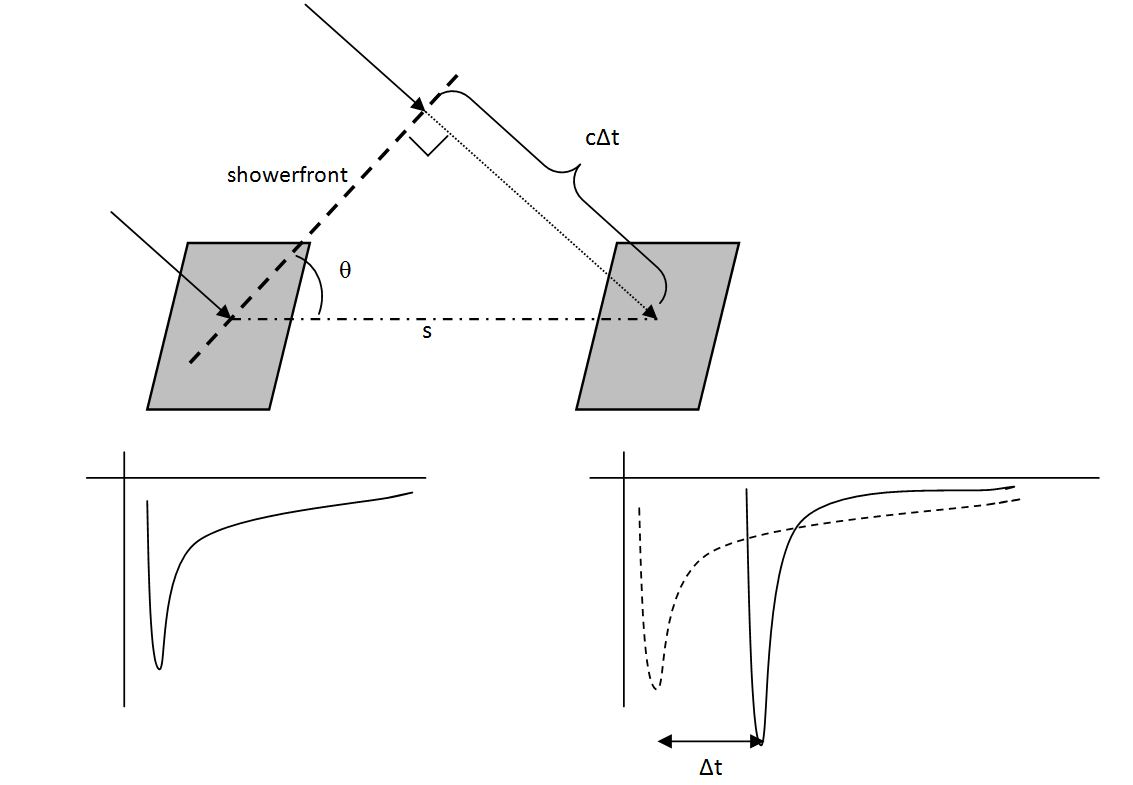
\includegraphics[scale=0.50]{showerfront2}
    \caption{Het \emph{shower front} (stippellijn) passeert de linker
             detector (grijs vlak) eerst. Een bepaalde tijd $\Delta t$
             later is het front bij de rechter detector. Het front reist
             met de lichtsnelheid en heeft dus schuin de afstand
             $c\Delta t$ afgelegd. Eronder staan de signalen die de
             detectoren meten, die in de rechter detector komt dus
             $\Delta t$ later, en kan een andere sterkte hebben.}
   \label{fig:showerfront2}
\end{figure}

\begin{figure}
    \centering
    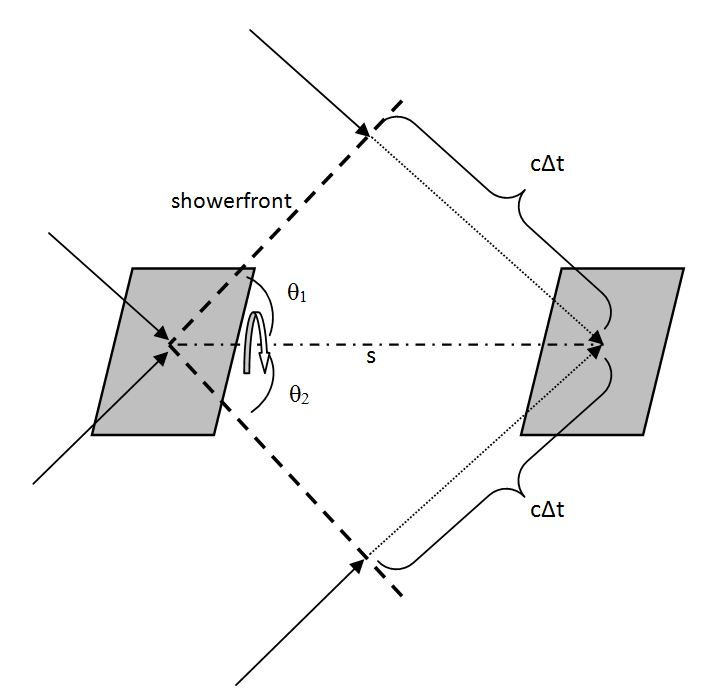
\includegraphics[scale=0.50]{showerfront3}
    \caption{Een shower vanuit richting $\theta_1$ heeft dezelfde
             $c\Delta t$ als een shower uit richting $\theta_2$, die
             vanuit de aarde lijkt te komen. Het inkomende \emph{shower
             front} is over alle hoeken tussen 0 en 2$\pi$ te roteren om
             s-as, waarbij de invalshoekhoek van de shower nog steeds
             klopt met bijhorende gemeten grootheden $s$ en $\Delta t$.
             Met twee platen kun je de richting vanwaar de shower komt
             dus niet bepalen.}
   \label{fig:showerfront3}
\end{figure}

Een richtingbepaling van een \emph{shower front} heeft minimaal drie
detectoren nodig. Wat logisch is, want om een vlak te tekenen zijn ook
minstens drie punten in de ruimte nodig. Om wel een reconstructie van
richting te maken is dus een derde detector nodig. Scholen, die een
station met twee detectoren hebben, kunnen ook een event gebruiken wat
een coïncidentie is met een event gemeten door een ander station in de
buurt, zodat een ander station het derde benodigde punt kan leveren. 


\section{Richting reconstructie met drie of meer detectoren}

In \figref{fig:frontthesis} is een situatie weergegeven van een vlak
\emph{shower front} waarvan de normaal (de shower as) een zenithoek
($\theta$) heeft met het (x,y)-vlak en een azimuthoek($\phi$) met de
x-as.

\begin{figure}
    \centering
    %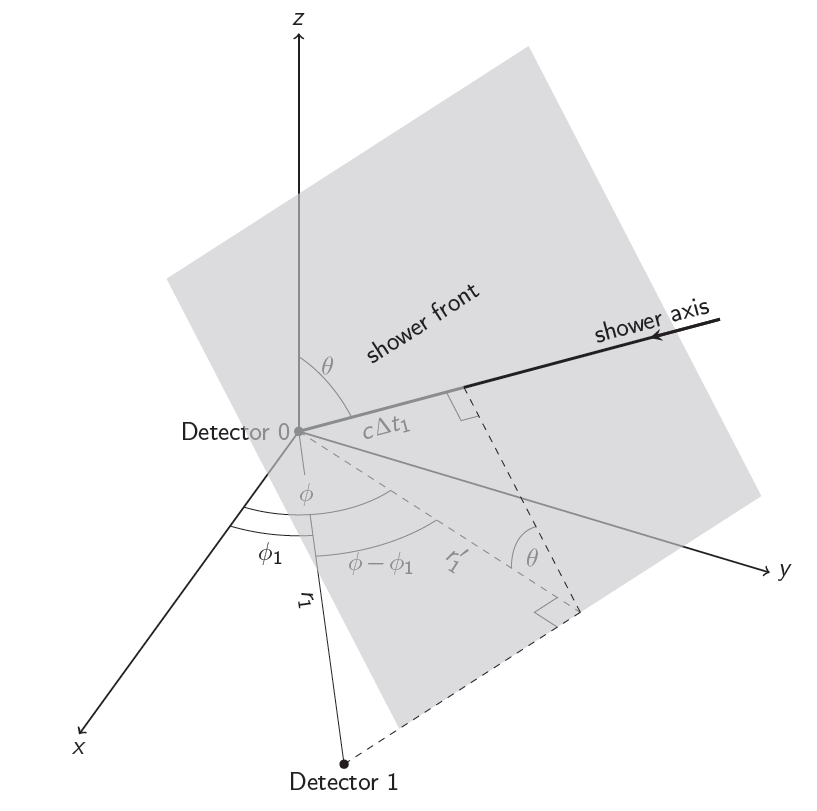
\includegraphics[scale=0.60]{front}
    \tdplotsetmaincoords{50}{115}
\pgfmathsetmacro{\axlen}{8}
\pgfmathsetmacro{\slen}{8}
\pgfmathsetmacro{\thetavec}{50}
\pgfmathsetmacro{\phivec}{70}
\pgfmathsetmacro{\phiovec}{30}
\pgfmathsetmacro{\rlen}{\slen * sin(\thetavec) / cos(\phivec - \phiovec)}
\pgfmathsetmacro{\splen}{\slen * sin(\thetavec) * sin(\thetavec)}
\pgfmathsetmacro{\ylen}{\slen * sin(\thetavec) * cos(\thetavec)}
\pgfmathsetmacro{\clen}{.5}

\begin{sansmath}
\begin{tikzpicture}[tdplot_main_coords, node distance=0pt, font=\sffamily]

% Set coordinates
\coordinate (O) at (0, 0, 0);
\tdplotsetcoord{S}{\slen}{\thetavec}{\phivec}
\tdplotsetcoord{D}{\rlen}{90}{\phiovec}
\tdplotsetcoord{S'}{\splen}{\thetavec}{\phivec}

% Draw axes
\draw[thick,->] (0, 0, 0) -- (\axlen, 0, 0) node[anchor=north]{$x$};
\draw[thick,->] (0, 0, 0) -- (0, \axlen, 0) node[anchor=west]{$y$};
\draw[thick,->] (0, 0, 0) -- (0, 0, \axlen) node[anchor=south]{$z$};

% Draw detector points
\fill (O) circle (2pt);
\node at (O) [anchor=east] {Detector 0};
\fill (D) circle (2pt);
\node at (D) [anchor=north] {Detector 1};

% Draw labelled lines
\draw[very thick] (O) -- (S');
\path (O) -- (S') node [midway,below,sloped] {$c \Delta t_1$};
\draw[dashed] (O) -- (Sxy) node [pos=.6,below,sloped] {$r'_1$};
\draw (O) -- (D) node [midway,below,sloped] {$r_1$};

% Draw phi angle arcs
\tdplotdrawarc{(O)}{2}{0}{\phivec}{above left,fill=white}{$\phi$}
\tdplotdrawarc{(O)}{2.5}{0}{\phiovec}{below}{$\phi_1$}
\tdplotdrawarc{(O)}{3}{\phiovec}{\phivec}{below}{$\phi - \phi_1$}

% Draw theta angle arcs and right angle square
\tdplotsetthetaplanecoords{\phivec}
\tdplotdrawarc[tdplot_rotated_coords]{(O)}{1.5}{0}{\thetavec}{above}{$\theta$}
\tdplotdrawarc[tdplot_rotated_coords]{(Sxy)}{1.5}{-90 + \thetavec}{-90}{below right}{$\theta$}

% Draw right angle square in rotated theta plane
\tdplotsetrotatedcoords{\phivec-90}{90}{90-\thetavec}
\draw[tdplot_rotated_coords] ($(S') + (\clen,0)$) -- +(0,-\clen) -- +(-\clen,-\clen);

% Draw right angle on ground
\tdplotsetrotatedcoords{\phivec-90}{0}{0}
\draw[tdplot_rotated_coords] ($(Sxy) + (\clen,0)$) -- +(0,-\clen) -- +(-\clen,-\clen);

% Draw shower front
\tdplotsetrotatedcoords{\phivec}{\thetavec}{0}
\fill[tdplot_rotated_coords,gray!50,opacity=.6] ($(S')-(\ylen,\ylen,0)$) -- +(2*\ylen,0,0) -- +(2*\ylen,2*\ylen,0) -- +(0,2*\ylen,0) -- cycle;
\path[tdplot_rotated_coords] ($(S')-(0,\ylen,0)$) -- +(0,2*\ylen,0) node [midway,sloped,above,inner sep=30] {shower front};

% Draw lines in front of shower front
\draw[very thick] (S') -- ($(S')!2.2!(S)$) node [near end,above,sloped] {shower axis};
\draw[very thick,-stealth] ($(S')!2.2!(S)$) -- ($(S')!1.6!(S)$);
\draw[dashed] (D) -- (Sxy);
\draw[dashed] (Sxy) -- (S');

\end{tikzpicture}
\end{sansmath}

    \caption{Het \emph{shower front} beweegt langs de \emph{shower as}
             bereikt detector 1. Een bepaalde tijd $\Delta t_1$ later is
             het front bij detector 0. Figuur overgenomen uit
             \cite{Fokkema}.}
  \label{fig:frontthesis}
\end{figure}

Het front passeert detector 1. Een bepaalde tijd $\Delta t_1$ later is
het front bij detector 0. Op een gelijke wijze kan ook een $\Delta t_2$
worden bepaald, het tijdsverschil tussen detector 0 en detector 2. Voor
de hoekreconstructie zijn minimaal drie detectoren nodig. In de
\hisparc-opstelling zijn dit òf de drie buitenste detectorplaten in een
station, òf drie stations die dezelfde EAS meten. Al eerder is een
dergelijke hoekreconstructie uitgevoerd met de volgende vergelijkingen,
afgeleid door D. Fokkema \cite{Fokkema}. Verdere uitleg over de richting
reconstructie van een shower is te vinden in
RouteNet\footnote{Te vinden op de site:
\url{http://www.hisparc.nl/docent-student/lesmateriaal/routenetpad/}}
onder "Richting reconstructie primair deeltje".

\begin{equation}
   \quad\tan(\phi) = \frac{r_1\Delta t_2\cos\phi_1-r_2\Delta t_1\cos\phi_2}
                          {r_2\Delta t_1\sin\phi_2-r_1\Delta t_2\sin\phi_1}
\end{equation}

\begin{equation}
    \quad\sin(\theta) = \frac{c\Delta t_1}{r_1\cos(\phi-\phi_1)}
\end{equation}

Hierin is $\phi_1$ de hoek tussen de detector 0 en detector 1 en $r_1$ de
afstand tussen deze detectoren. $\phi_2$ is de hoek tussen detector 0 en
detector 2 en $r_2$ de afstand tussen deze detectoren. $c$ is de
lichtsnelheid.

\begin{figure}
    \centering
    %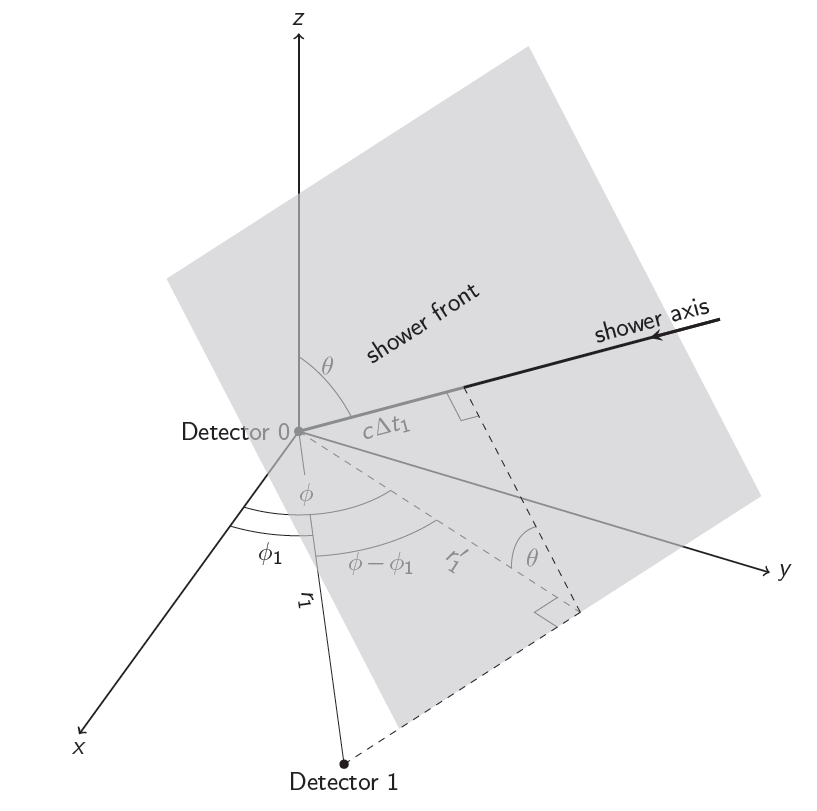
\includegraphics[scale=0.60]{front}
    % !TeX root = thesis.tex

\begin{tikzpicture}
    [ font=\sffamily, x=.75cm, y=.75cm,
      hisparc/.style={draw},
    ]
    \foreach \sx / \sy / \angle in {-5/0/90, 5/0/-90, 0/2.89/0, 0/8.66/0} {
        \begin{scope}[hisparc, shift={(\sx,\sy)}, rotate=\angle]
            \draw[rounded corners=2.25pt]
                (-.4, .7) .. controls (0, .75) ..  (.4, .7) -- 
                (.35, -1.7) ..  controls(0, -1.72) ..  (-.35, -1.7) --
                cycle;
            \draw (-.25, .5) rectangle (.25, -.5);
            \draw (-.25, -.5) -- (-.02, -1) --(.02, -1) -- (.25, -.5);
            \fill (-.02, -1) rectangle (.02, -1.2);
            \draw (0, 0) circle (.1);
        \end{scope}
    }
    \draw[fill] (0, 0) circle (.10) node [below] {GPS};
    \node[color=gray] at (-.75, 8.66) {\Large 1};
    \node[color=gray] at (-.75, 2.89) {\Large 2};
    \node[color=gray] at (-5, .75) {\Large 3};
    \node[color=gray] at (5, .75) {\Large 4};

    \coordinate (A) at (-5, 0);
    \coordinate (B) at (5, 0);
    \coordinate (A') at ($ (A)!.8cm!-90:(B) $);
    \coordinate (B') at ($ (B)!.8cm!90:(A) $);
    \draw (A) -- ($ (A)!1.1!(A') $);
    \draw (B) -- ($ (B)!1.1!(B') $);
    \draw[<->] (A') -- (B') node [midway, below] {\SI{10}{\meter}};

    \coordinate (D) at (0, 8.66);
    \coordinate (C') at ($ (A)!.8cm!90:(D) $);
    \coordinate (D') at ($ (D)!.8cm!-90:(A) $);
    \draw (A) -- ($ (A)!1.1!(C') $);
    \draw (D) -- ($ (D)!1.1!(D') $);
    \draw[<->] (C') -- (D') node [midway, above, sloped] {\SI{10}{\meter}};

    \coordinate (E) at (0, 0);
    \coordinate (F) at (0, 2.89);
    \coordinate (D'') at ($ (D)!.8cm!90:(E) $);
    \coordinate (E') at ($ (E)!.8cm!-90:(D) $);
    \coordinate (F') at ($ (F)!.8cm!-90:(D) $);
    \draw (E) -- ($ (E)!1.1!(E') $);
    \draw (F) -- ($ (F)!1.1!(F') $);
    \draw (D) -- ($ (D)!1.1!(D'') $);
    \draw[<->] (E') -- (F') node [midway, below, sloped]
        {\SI{2.89}{\meter}};
    \draw[<->] (F') -- (D'') node [midway, below, sloped]
        {\SI{5.77}{\meter}};

    \draw[dashed,gray] (A) -- (B);
    \draw[dashed,gray] (A) -- (D);
    \draw[dashed,gray] (A) -- (F);
    \draw[dashed,gray] (B) -- (D);
    \draw[dashed,gray] (B) -- (F);
    \draw[dashed,gray] (F) -- (D);
\end{tikzpicture}

    \caption{Opbouw van een vier detectorstation. De detectoren op de
             hoekpunten liggen op een gelijkzijdige driehoek met zijdes
             van \SI{10}{\meter}. De detectoren zijn ook genummerd, dit
             wordt bepaald door hoe ze aan de \hisparc electronica
             verbonden zijn.}
    \label{fig:stationlayout} 
\end{figure}

\textbf{Opdracht 1} Richting bepaling van station 501. Bekijk tabel
\ref{tab:arrival} met een meting van de aankomsttijden van een
\emph{shower front} bij drie detectoren van één station. De
aankomsttijden zijn gegeven in ns. De detectoren van het station zijn
opgesteld zoals in \figref{fig:stationlayout}.\\
Bereken hoek $\phi$ en hoek $\theta$ met behulp van de gevens in tabel
\ref{tab:arrival}.

\begin{center}
    \rule{\textwidth}{0.3mm}
    \\
    \rule{\textwidth}{0.3mm}
    \\
    \rule{\textwidth}{0.3mm}
    \\
    \rule{\textwidth}{0.3mm}
    \\
\end{center}

\begin{table}
    \centering
    \begin{tabular}{ |l |l |}    
        \hline
        Detector & Aankomsttijd \\ 
        \hline
        1 & \SI{0.0}{\nano\second} \\
        \hline
        3 & \SI{7.6}{\nano\second} \\
        \hline
        4 & \SI{9.2}{\nano\second} \\ 
        \hline
    \end{tabular}
    \caption{Aankomsttijden van een shower gedecteerd door station 501.
             Detector 2 is weggelaten om dat het nauwkeuriger is de
             hoekpunten van de driehoek te gebruiken.}
    \label{tab:arrival}
\end{table}
 

\begin{thebibliography}{9}
    \bibitem{Fokkema}
        D.B.R.A. Fokkema, \emph{The \hisparc Experiment, data
        acquisition and reconstruction of shower direction}, PhD. thesis
        2012
\end{thebibliography}

\end{document}
